\documentclass{article}
\usepackage{listings}
\usepackage{mathtools, amssymb}
\usepackage{tikz}
\usepackage{enumitem}
\usepackage[margin=1in]{geometry}

\title{CSE 130 Homework 3}
\author{Jack Shi - A92122910\\
				Wyatt Guidry - A12994977\\
			  Austin Coleman - A12888539}
\date{Feb 9, 2018}

\begin{document}
\maketitle

% 1
\section{Type embodiment and parametricity}
% 1.1
\subsection{The Algebra of Datatypes}
\begin{enumerate}
	% 1.
	\item How many inhabitants does \texttt{Animal} have? Give an example\\
		\textbf{Answer:} $|Animal|=3$
		\begin{lstlisting}
		myCat = Cat :: Animal
		\end{lstlisting} 

	% 2.
	\item How many inhabitants does \texttt{AnimalPair} have? Give an example\\
		\textbf{Answer:} $|AnimalPair|=9$
		\begin{lstlisting}
		myCatPair = AnimalPair myCat myCat :: AnimalPair
		\end{lstlisting} 

	% 3.
	\item How many inhabitants does \texttt{Maybe Animal} have? Give an example\\
		\textbf{Answer:} $|Maybe Animal|=4$
		\begin{lstlisting}
		Just Cat
		\end{lstlisting} 

	% 4.
	\item How many inhabitants does \texttt{Maybe} have? Give your
		answer in terms of a.\\
		\textbf{Answer:} $|Maybe|= |a|+1$

	% 5.
	\item How many inhabitants does \texttt{Pair a b} have? Give your
		answer in terms of a and b.\\
		\textbf{Answer:} $|Pair a b|=|a|\cdot|b|$

	% 6.
	\item How many inhabitants does \texttt{Either (Maybe Animal)
		(Pair (Pair Animal Animal) Animal)} have?\\
		\textbf{Answer:} $|$Either (Maybe Animal) (Pair (Pair Animal Animal)
		Animal)$|=4 + ((3\cdot 3)\cdot 3)=31$
		\begin{lstlisting}
		\end{lstlisting} 

\end{enumerate}

% 1.2
\subsection{Types and Lambda Calculus}
\begin{enumerate}
	% 1.
	\item $a \rightarrow a$\\
		\textbf{Answer:} 1 function. $\lambda x.x$

	% 2.
	\item $a \rightarrow b$\\
		\textbf{Answer:} $\infty$ functions. $\lambda x.e \mid type(e)\neq type(x)$

	% 3.
	\item $a \rightarrow b \rightarrow a$\\
		\textbf{Answer:} 1 function. $\lambda xy.x$

	% 4.
	\item $a \rightarrow b \rightarrow b$\\
		\textbf{Answer:} 1 function. $\lambda xy.y$

	% 5.
	\item $(a \rightarrow b \rightarrow c) \rightarrow (a \rightarrow b)
		\rightarrow a \rightarrow c$\\
		\textbf{Answer:} 1 function. $\lambda fga.f\ a\ (g\ a)$

	% 6.
	\item $a \rightarrow \mathbb{Z}_6$\\
		\textbf{Answer:} 6 function. 
		\begin{align*}
			&\lambda x.0\\
			&\lambda x.1\\
			&\lambda x.2\\
			&\lambda x.3\\
			&\lambda x.4\\
			&\lambda x.5
		\end{align*}

\end{enumerate}

% 1.3
\subsection{Type Tetris}

\begin{align*}
	(\$)&::(a\rightarrow b) \rightarrow a \rightarrow b\\
	(.)&::(b\rightarrow c) \rightarrow (a \rightarrow b) \rightarrow (a \rightarrow c)\\
	flip&::(a\rightarrow b \rightarrow c) \rightarrow (b\rightarrow a \rightarrow c)\\
	map&::(a\rightarrow b) \rightarrow [a] \rightarrow [b]\\
	concat&::[[a]] \rightarrow [b]
\end{align*}

\begin{enumerate}
	% 1.
	\item Give a definition for $bog::(a \rightarrow [b]) \rightarrow [a]
		\rightarrow [b]$\\
		\textbf{Answer:} 
			\begin{lstlisting}
				bog::concat.map
			\end{lstlisting} 
	% 2.
	\item \textbf{WIP}Give a definition for $zog::a \rightarrow [a \rightarrow b] \rightarrow [b]$\\
		\textbf{Answer:} 
			\begin{lstlisting}
				zog::
			\end{lstlisting} 

\end{enumerate}

% 2
\section{Type Inference}
% 2.1
\subsection{Infer the type of \texttt{reverse:}}
\setcounter{equation}{-1}
\textbf{Answer:}\\
\begin{lstlisting}
	reverse [] = []
\end{lstlisting}

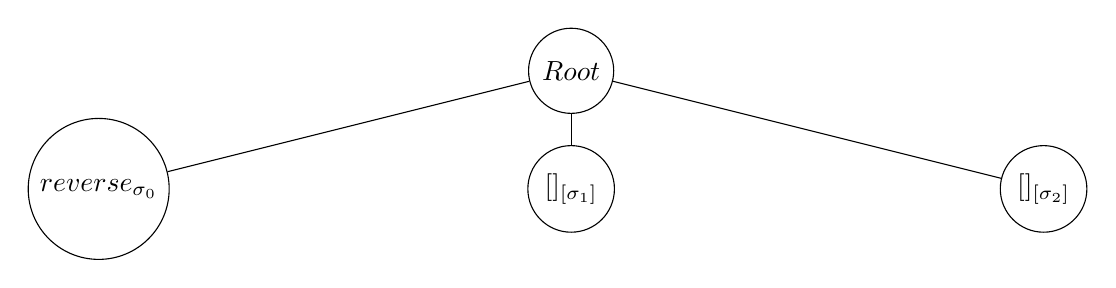
\begin{tikzpicture}[level/.style={sibling distance=60mm/#1}]
	\node [circle,draw] (root) {$Root$}
		child {node [circle,draw] (reverse) {$reverse_{\sigma_0}$}}
		child {node [circle,draw] (argList) {$[]_{[\sigma_1]}$}}
		child {node [circle,draw] (expList) {$[]_{[\sigma_2]}$}};
\end{tikzpicture}\\

\begin{equation}
\sigma_0 = [\sigma_1] \rightarrow [\sigma_2]
\end{equation}

\begin{lstlisting}
	reverse (x:xs) = reverse xs ++ [x]
	               = ((++) (reverse xs)) [x]
\end{lstlisting}

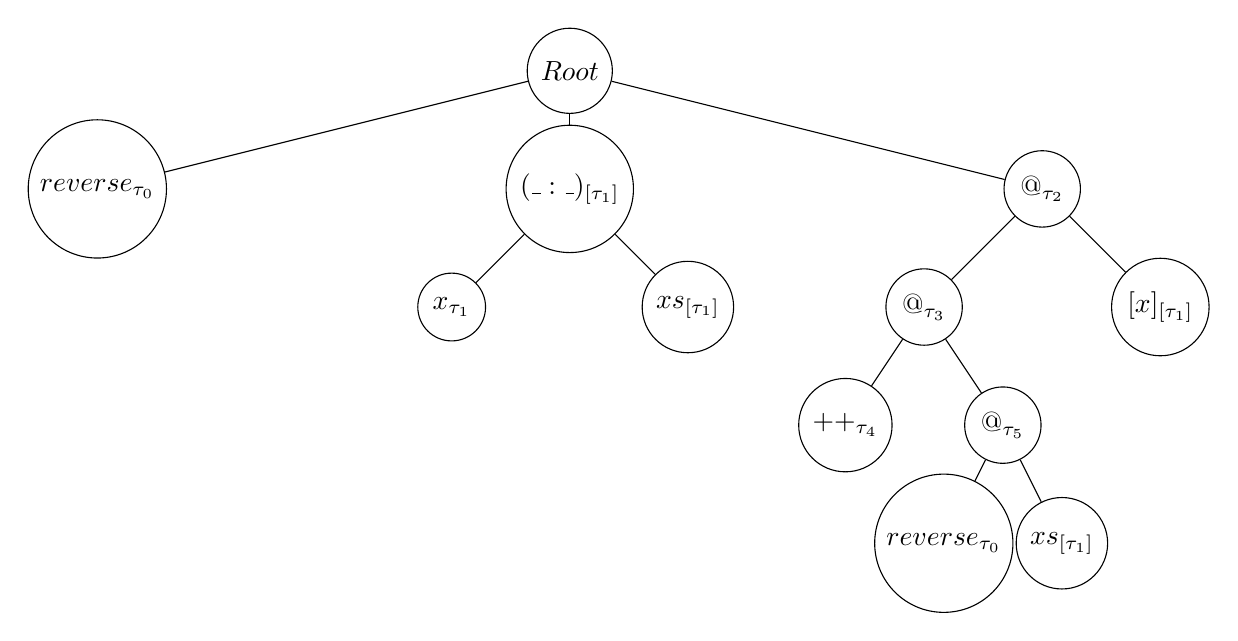
\begin{tikzpicture}[level/.style={sibling distance=60mm/#1}]
	\node [circle,draw] (root) {$Root$}
		child {node [circle,draw] (reverseArg) {$reverse_{\tau_0}$}}
		child {node [circle,draw] (con) {$(\_:\_)_{[\tau_1]}$}
			child {node [circle,draw] (xArg) {$x_{\tau_1}$}}
			child {node [circle,draw] (xsArg) {$xs_{[\tau_1]}$}}
		}
		child {node [circle,draw] (applyRevConcat) {$@_{\tau_2}$}
			child {node [circle,draw] (applyConcat) {$@_{\tau_3}$}
				child {node [circle,draw] (applyConcat2) {$++_{\tau_4}$}}
				child {node [circle,draw] (applyRev) {$@_{\tau_5}$}
					child {node [circle,draw] (reverse) {$reverse_{\tau_0}$}}
					child {node [circle,draw] (xs) {$xs_{[\tau_1]}$}}
				}
			}
			child {node [circle,draw] (xListExp) {$[x]_{[\tau_1]}$}}
		};
\end{tikzpicture}

\begin{align}
	\tau_0 &= [\tau_1] \rightarrow \tau_2\\
	\tau_0 &= [\tau_1] \rightarrow \tau_5\\
	\tau_4 &= \tau_5 \rightarrow \tau_3\\
	\tau_3 &= [\tau_1] \rightarrow \tau_2\\
	++ &:: [a] \rightarrow [a] \rightarrow [a]
\end{align}

\begin{center} Unify(1, 2) \end{center}
\begin{equation}  
	[\tau_1] \rightarrow \tau_2 = [\tau_1] \rightarrow \tau_5 \Rightarrow
	\tau_5 = \tau_2 \end{equation}

\begin{center} Subsitute 6 and 4 into 3 \end{center}
\begin{equation}  
	\tau_4 = \tau_2 \rightarrow ([\tau_1] \rightarrow \tau_2) \end{equation}  

\begin{center} Unify(5, 7) \end{center}
\begin{equation}  
	\tau_2 \rightarrow ([\tau_1] \rightarrow \tau_2) = [a] \rightarrow [a]
	\rightarrow [a] \Rightarrow \tau_2 = [\tau_1]
\end{equation}  


\begin{center} \textbf{Solution: }\end{center}
\begin{equation*}  
	\tau_0 = [\tau_1] \rightarrow [\tau_1] \end{equation*}  

% 2.2
\subsection{Infer the type of \texttt{foldl:}}
\setcounter{equation}{-1}
\textbf{Answer:}\\
\begin{lstlisting}
	foldl f acc [] = acc
\end{lstlisting}

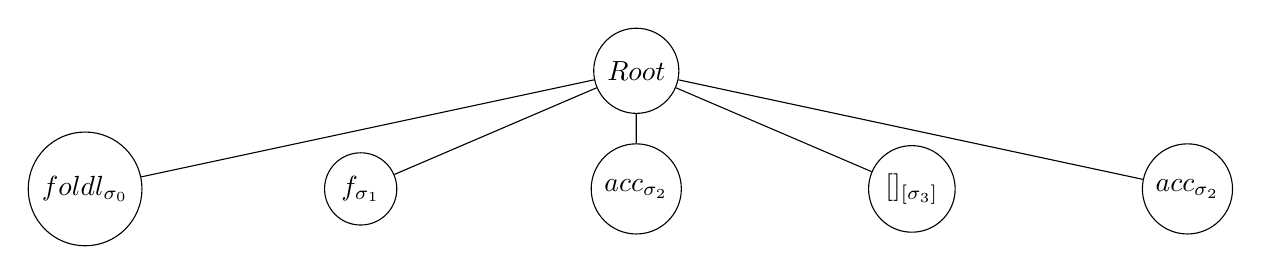
\begin{tikzpicture}[level/.style={sibling distance=35mm/#1}]
	\node [circle,draw] (root) {$Root$}
		child {node [circle,draw] (fl) {$foldl_{\sigma_0}$}}
		child {node [circle,draw] (argf) {$f_{\sigma_1}$}}
		child {node [circle,draw] (argacc) {$acc_{\sigma_2}$}}
		child {node [circle,draw] (argls) {$[]_{[\sigma_3]}$}}
		child {node [circle,draw] (expacc) {$acc_{\sigma_2}$}};
\end{tikzpicture}\\

\begin{equation}
	\sigma_0 = \sigma_1 \rightarrow \sigma_2 \rightarrow [\sigma_3] \rightarrow
\sigma_2
\end{equation}

\begin{lstlisting}
	foldl f acc (x:xs) = foldl f (f acc x) xs
	                   = ((foldl f) ((f acc) x)) xs
\end{lstlisting}

\begin{tikzpicture}[level/.style={sibling distance=35mm/#1, 
																	level distance=2cm},
										level 3/.style={sibling distance=30mm},
										level 4/.style={sibling distance=15mm},
										level 5/.style={sibling distance=15mm}]
	\node [circle,draw] (root) {$Root$}
		child {node [circle,draw] (fl) {$foldl_{\tau_0}$}}
		child {node [circle,draw] (argf) {$f_{\tau_1}$}}
		child {node [circle,draw] (argacc) {$acc_{\tau_2}$}}
		child {node [circle,draw] (argls) {$(\_:\_)_{[\tau_3]}$}
			child {node [circle,draw] (argvx) {$x_{\tau_3}$}}
			child {node [circle,draw] (argxs) {$xs_{[\tau_3]}$}}
		}
		child {node [circle,draw] (exapp1) {$@_{\tau_4}$}
			child {node [circle,draw] (exapp2) {$@_{\tau_5}$}
				child {node [circle,draw] (exapp3) {$@_{\tau_6}$}
					child {node [circle,draw] (exfoldl) {$foldl_{\tau_0}$}}
					child {node [circle,draw] (exf) {$f_{\tau_1}$}}
				}
				child {node [circle,draw] (exapp4) {$@_{\tau_7}$}
					child {node [circle,draw] (exapp5) {$@_{\tau_{8}}$}
						child {node [circle,draw] (exf2) {$f_{\tau_1}$}}
						child {node [circle,draw] (exacc) {$acc_{\tau_2}$}}
					}
					child {node [circle,draw] (exx) {$x_{\tau_3}$}}
				}
			}
			child {node [circle,draw] (expxs) {$xs_{[\tau_3]}$}}
		};
\end{tikzpicture}\\

\begin{align}
	\tau_0 &= \tau_1 \rightarrow \tau_2 \rightarrow [\tau_3] \rightarrow \tau_4\\
	\tau_5 &= [\tau_3] \rightarrow \tau_4\\
	\tau_6 &= \tau_7 \rightarrow \tau_5\\
	\tau_0 &= \tau_1 \rightarrow \tau_6\\
	\tau_8 &= \tau_3 \rightarrow \tau_7\\
	\tau_1 &= \tau_2 \rightarrow \tau_8
\end{align}

\begin{center} Unify(1, 4) \end{center}
\begin{equation}  
	\tau_1 \rightarrow \tau_2 \rightarrow [\tau_3] \rightarrow \tau_4 =
	\tau_1 \rightarrow \tau_6  \Rightarrow 
	\tau_6 = \tau_2 \rightarrow [\tau_3] \rightarrow \tau_4 \end{equation}

\begin{center} Subsitute 6 to 1\end{center}
\begin{equation}  
	\tau_0 = (\tau_2 \rightarrow \tau_8) \rightarrow \tau_2 \rightarrow [\tau_3]
	\rightarrow \tau_4
\end{equation}

\begin{center} Subsitute 5 to 8\end{center}
\begin{equation}  
	\tau_0 = (\tau_2 \rightarrow \tau_3 \rightarrow \tau_7) \rightarrow \tau_2
	\rightarrow [\tau_3] \rightarrow \tau_4
\end{equation}

\begin{center} Subsitute 2 to 3\end{center}
\begin{equation}  
	\tau_6 = \tau_7 \rightarrow ([\tau_3] \rightarrow \tau_4)\\
\end{equation}

\begin{center} Unify(7, 10) \end{center}
\begin{equation}  
\tau_7 \rightarrow ([\tau_3] \rightarrow \tau_4) = \tau_2 \rightarrow [\tau_3]
\rightarrow \tau_4  \Rightarrow \tau_7 = \tau_2
\end{equation}

\begin{center} Subsitute 11 to 9\end{center}
\begin{equation}  
\tau_0 = (\tau_2 \rightarrow \tau_3 \rightarrow \tau_2) \rightarrow \tau_2
	\rightarrow [\tau_3] \rightarrow \tau_4
\end{equation}

\begin{center} Unify(0, 12) \end{center}
\begin{equation}  
(\tau_2 \rightarrow \tau_3 \rightarrow \tau_2) \rightarrow \tau_2
	\rightarrow [\tau_3] \rightarrow \tau_4 = \sigma_1 \rightarrow \sigma_2
	\rightarrow [\sigma_3] \rightarrow \sigma_2 \Rightarrow \tau_4 = \tau_2
\end{equation}

\begin{center} Subsitute 13 to 12\end{center}
\begin{equation}  
\tau_0 = (\tau_2 \rightarrow \tau_3 \rightarrow \tau_2) \rightarrow \tau_2
	\rightarrow [\tau_3] \rightarrow \tau_2
\end{equation}

\begin{center} \textbf{Solution: }\end{center}
\begin{equation*}  
\tau_0 = (\tau_2 \rightarrow \tau_3 \rightarrow \tau_2) \rightarrow \tau_2
	\rightarrow [\tau_3] \rightarrow \tau_2
\end{equation*}  

\end{document}

